\documentclass{article}
\linespread{0.7}
\usepackage[a4paper, margin=3mm, landscape]{geometry}
\usepackage{multicol}
\usepackage{xcolor}
\usepackage{enumitem}
\usepackage{amsmath}
\usepackage{amsfonts}
\usepackage{listings}
\usepackage{soul}
\usepackage{graphicx}

\pdfinfo{
    /Title (ee3801-cheatsheet.pdf)
    /Creator (TeX)
    /Producer (pdfTeX 1.40.0)
    /Author (Vincent Pang)
    /Subject (template)
    /Keywords (cheatsheet, pdf, ee3801)
}

\graphicspath{ {./img/} }

\pagestyle{empty}
\setcounter{secnumdepth}{0}
\setlength{\columnseprule}{0.25pt}

% Redefine section commands to use less space
\makeatletter
\renewcommand{\section}{\@startsection{section}{1}{0mm}%
    {-1ex plus -.5ex minus -.2ex}%
    {0.5ex plus .2ex}%x
{\normalfont\large\bfseries}}
\renewcommand{\subsection}{\@startsection{subsection}{2}{0mm}%
    {-1explus -.5ex minus -.2ex}%
    {0.5ex plus .2ex}%
{\normalfont\normalsize\bfseries}}
\renewcommand{\subsubsection}{\@startsection{subsubsection}{3}{0mm}%
    {-1ex plus -.5ex minus -.2ex}%
    {1ex plus .2ex}%
{\normalfont\small\bfseries}}%
\makeatother

% Adjust spacing for all itemize/enumerate
\setlength{\leftmargini}{0.5cm}
\setlength{\leftmarginii}{0.5cm}
\setlist[itemize,1]{leftmargin=2mm,labelindent=1mm,labelsep=1mm}
\setlist[itemize,2]{leftmargin=2mm,labelindent=1mm,labelsep=1mm}

% Font
\renewcommand{\familydefault}{\sfdefault}

% Define colors for math formulas
\definecolor{myblue}{cmyk}{1,.72,0,.38}
\everymath\expandafter{\the\everymath \color{myblue}}

% Custom command for keywords
\definecolor{highlight}{RGB}{251,243,218}
\newcommand{\keyword}[2][]{\sethlcolor{highlight}\hl{\textbf{#2}} #1 - }
\newcommand{\ilkeyword}[1]{\sethlcolor{highlight}\hl{\textbf{#1}}}

% Define colors and style for code
\definecolor{codegreen}{rgb}{0,0.6,0}
\definecolor{codegray}{rgb}{0.5,0.5,0.5}
\definecolor{codered}{HTML}{CC241D}
\definecolor{backcolor}{rgb}{0.95,0.95,0.95}
\lstdefinestyle{codestyle}{
    backgroundcolor = \color{backcolor},
    commentstyle = \color{codegray},
    keywordstyle = \color{codered},
    stringstyle = \color{codegreen},
    basicstyle = \ttfamily,
    breakatwhitespace = false,
    showstringspaces = false,
    breaklines = true,
    showtabs = false,
    tabsize = 2
}
\lstset{style = codestyle}

% -----------------------------------------------------------------------
\begin{document}
\begin{multicols*}{3}
\footnotesize

% Title box
\begin{center}
    \fbox{
        \parbox{0.8\linewidth}{
            \centering \textcolor{black}{
                {\Large\textbf{EE3801 Cheatsheet}} \\
                \normalsize{Intro to Data Engineering}} \\
                {\footnotesize \textcolor{gray}{github.com/securespider}}
        }
    }
\end{center}
\section{01.1 Intro}
\subsection{Data science vs engineering}
\begin{itemize}
	\item \keyword{Science}{Learn, optimise, analytics, aggregate and labelling}
	\item \keyword{Engineering}{Cleaning, data storage, logging, sensors, pipelines}
\end{itemize}
\subsection{Data structure}
\subsubsection{Unstructured data}
\begin{itemize}
	\item{Chaotic no order to data}
\end{itemize}
\subsubsection{Structured data}
\begin{itemize}
	\item Data stored access in the same format
\end{itemize}
\subsubsection{Semi structured data}
\begin{itemize}
	\item Can contain both forms of data 
	\item Some structure but not all data points follow same format
\end{itemize}
\subsection{Big data}
\begin{description}
	\item[Volume, Variety, Variability]
	\item[Velocity]{High rate of data generation}
	\begin{itemize}
		\item Must create a robust and scalable pipeline
	\end{itemize}
\end{description}
\subsection{Raw Data}
\begin{itemize}
	\item Tend to have gaps
\end{itemize}
\subsubsection{Data wrangling}
Used to understand raw data
\begin{description}
	\item[Discovery]{Understand what is in your data}
	\item[Structure]
	\item[Cleaning]{Dealing with gaps (nulls), outliers, formatting bugs}
	\item[Enrichment]{Derive other data from other information/ additional data augmentation (feature selection)}
	\item[Validation]{Verify data quality, sources}
	\item[Publishing]{Give data scientist}
\end{description}
\subsection{Process}
\begin{description}
	\item[Extraction]{Retrieve raw data from unstructured pool and migrate to temp repo}
	\item[Transformation]{Structure enrich and convert raw data}
	\item[Loading]{Loading structured data into data warehouse}
\end{description}
\subsubsection{Data warehouse}
Decision support system storing historical data from organisations
\subsubsection{Data Pipeline}
\begin{itemize}
	\item Processing underlying raw data in ordered sequence of steps
\end{itemize}

\section{01.2 Data Pipelines}
\subsection{Considerations}
\subsubsection{Big data}
\begin{description}
	\item[Velocity]{Streaming, captured and processed in real time}
	\item[Volume]{Scalable wrt time}
	\item[Variety]{Recognise and process diff formats}
\end{description}
\subsubsection{Business}
\begin{itemize}
	\item Handling streaming data?
	\item How much data to expect (Time horizon/how much storage consumed)
	\item What type/how much processing in DP
	\item Where is data source? Need micro-services?
\end{itemize}
\subsection{Architecture}
\subsubsection{Batch-based DP}
\begin{itemize}
	\item Analysis of data that has been stored over a period of time
	\item $N$ independent tasks to process with $k$ stages
	\item Each stage takes max of $T$ time process input
	\item Diff stage can operate concurrently
	\item $t(N,k) = T\times(N+k-1)$
\end{itemize}
\subsubsection{Streaming-based DP}
\begin{itemize}
	\item Processing as data flows through system
	\item Logging and persistent result storage
\end{itemize}
\subsubsection{Lambda Architecture}
\begin{itemize}
	\item Combination of batch and streaming
	\item Separate processing engine for "batch" and "speed" layers combining in "service" layer
	\item Accounts for real-time streaming and historical batch analysis
	\item Encourage raw data storage and create new dst for queries
	\item Min errors for both layers reliably at fast speeds
\end{itemize}
\subsubsection{Kappa Architecture}
\begin{itemize}
	\item Replay data and process both layers in same single stream processing engine
	\item Good for big data architecture with cheaper hardware and focus on stream
\end{itemize}
\subsection{Design}
\begin{enumerate}
	\item Identify application and decide if DP needed
	\item Identify DP category (architecture)
	\item Understand working mechanism, parameters/variables
\end{enumerate}
\section{04. Big Data Computing Technology Platform}
\subsection{Packaging}
\begin{description}
	\item[Compact]{Nodes closely packaged in racks where nodes are not attached to peripherals}
	\item[Slack]{Nodes attached to peripherals connected remotely}
\end{description}
\subsubsection{Interconnection Medium}
Considerations
\begin{enumerate}
	\item Available link speeds
	\item Message Passing Interface (MPI) latency
	\item Network processor/routing mechanism/flow control
	\item Differing network topologies
\end{enumerate}
\textbf{Self routing/Destination tag} \\
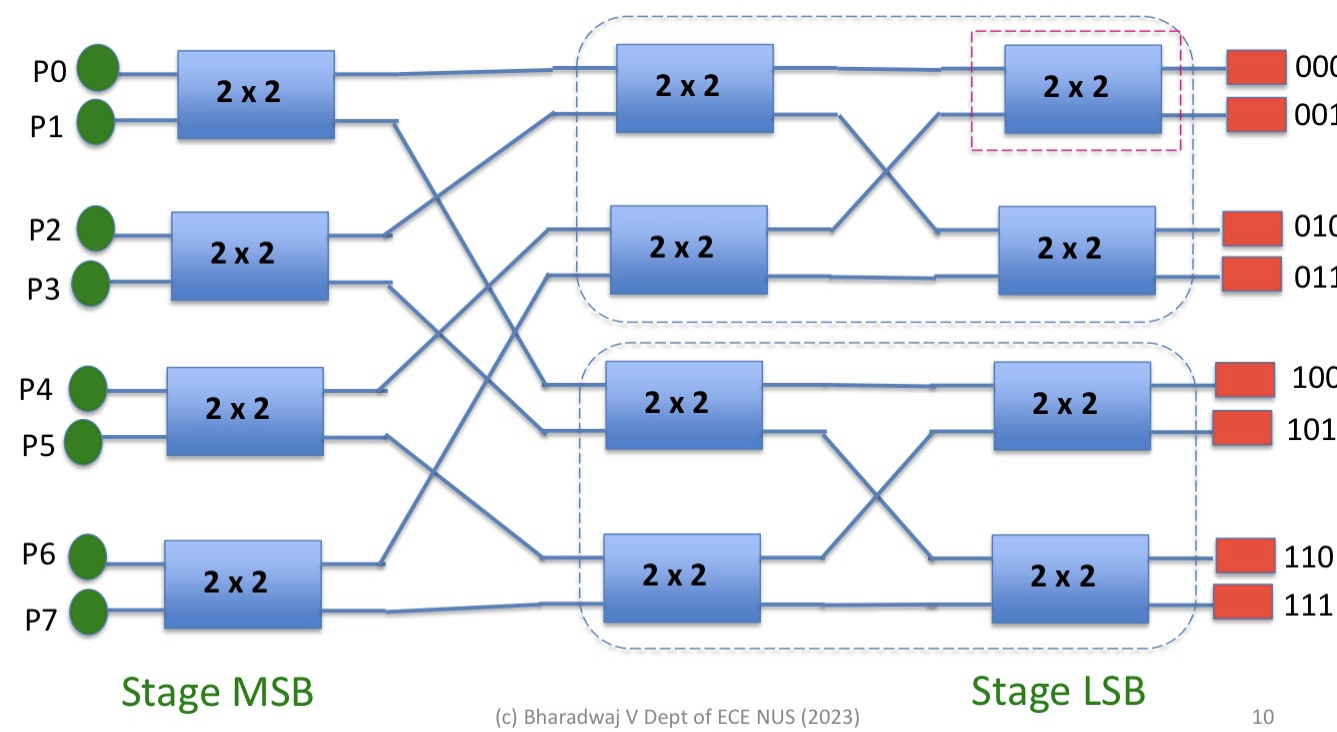
\includegraphics[scale=0.2]{self-routing}
\begin{itemize}
	\item Every processor can be routed to every memory without external controller
	\item Switch should know what stage it is in to know which bit to look for
	\item Bit of stage defines which output interface it leaves (0-above, 1-below)
\end{itemize}
\subsection{Control}
\begin{description}
	\item[Centralized]{Nodes owned, ctrl by central operator}
	\begin{itemize}
		\item Easy to manage 
		\item Used by compact and slack clusters
	\end{itemize}
	\item[Decentralized]{Nodes have individual owners}
	\begin{itemize}
		\item Minimize coupling and can be used w many OS
		\item Only slack can have
	\end{itemize}
\end{description}
\subsubsection{Homogeneity}
\begin{description}
	\item[Homogeneous]
	\item[Heterogeneous]
\end{description}
\subsection{Resource sharing}
\begin{description}
	\item[Share-nothing]{Each node do itself and send results together after}
	\item[Shared-disk]{When one node fail the other take over}
	\begin{itemize}
		\item Fault tolerance via checkpoints
	\end{itemize}
	\item[Shared-memory]{Connected via SScalable Coherence Interface ring}
	\begin{itemize}
		\item All common data/instruction written in shared space
	\end{itemize}
\end{description}
\end{multicols*}
\end{document}
